%%%%%%%% ICML 2023 EXAMPLE LATEX SUBMISSION FILE %%%%%%%%%%%%%%%%%

\documentclass{article}

% Recommended, but optional, packages for figures and better typesetting:
\usepackage{microtype}
\usepackage{graphicx}

\usepackage[position=top]{subfig}
\usepackage{subcaption}
\usepackage{booktabs} % for professional tables

% hyperref makes hyperlinks in the resulting PDF.
% If your build breaks (sometimes temporarily if a hyperlink spans a page)
% please comment out the following usepackage line and replace
% \usepackage{icml2023} with \usepackage[nohyperref]{icml2023} above.
\usepackage{hyperref}


% Attempt to make hyperref and algorithmic work together better:
\newcommand{\theHalgorithm}{\arabic{algorithm}}

% Use the following line for the initial blind version submitted for review:
\usepackage{icml2023}

% If accepted, instead use the following line for the camera-ready submission:
% \usepackage[accepted]{icml2023}

% For theorems and such
\usepackage{amsmath}
\usepackage{amssymb}
\usepackage{mathtools}
\usepackage{amsthm}

% if you use cleveref..
\usepackage[capitalize,noabbrev]{cleveref}

%%%%%%%%%%%%%%%%%%%%%%%%%%%%%%%%
% THEOREMS
%%%%%%%%%%%%%%%%%%%%%%%%%%%%%%%%
\theoremstyle{plain}
\newtheorem{theorem}{Theorem}[section]
\newtheorem{proposition}[theorem]{Proposition}
\newtheorem{lemma}[theorem]{Lemma}
\newtheorem{corollary}[theorem]{Corollary}
\theoremstyle{definition}
\newtheorem{definition}[theorem]{Definition}
\newtheorem{assumption}[theorem]{Assumption}
\theoremstyle{remark}
\newtheorem{remark}[theorem]{Remark}

% Todonotes is useful during development; simply uncomment the next line
%    and comment out the line below the next line to turn off comments
%\usepackage[disable,textsize=tiny]{todonotes}


\usepackage{algorithm}
\usepackage{algorithmic}
\usepackage{multirow}
\usepackage[textsize=tiny]{todonotes}
\usepackage{newfloat}
\usepackage{listings}
\usepackage{amsmath}
\usepackage{setspace}
% placeholders
\usepackage{color}
\def\yy#1{{\color{red}\textbf{yy: #1}}}
\def\at#1{{\color{green}\textbf{at: #1}}}
\def\sk#1{{\color{blue}{\textbf{SK: #1}}}}

% Math
\DeclareMathOperator*{\argmin}{\arg\!\min}
\DeclareMathOperator*{\argmax}{\arg\!\max}
\def\vec#1{{\bm #1}}
\def\tnull{{\text{null}}}
\def\vec#1{{\bm #1}}
\def\diag{\text{diag}}
\def\mat#1{\mathbf{#1}}
\def\Xmat{{\bm X}}
\def\Exp{{\mathbb E}}
\def\Var{\text{Var}}
\def\ErdosRenyi{{Erd\H{o}s-R\'{e}nyi}\xspace}
\def\given{\mid}
\newcommand{\Var}{\mathrm{Var}}



\usepackage[group-separator={,}]{siunitx}
\usepackage{booktabs}

%\doublespacing
% The \icmltitle you define below is probably too long as a header.
% Therefore, a short form for the running title is supplied here:
\icmltitlerunning{Debiasing graph neural networks for missing link prediction}

\begin{document}

\twocolumn[
\icmltitle{Debiasing graph neural networks for link prediction}

% It is OKAY to include author information, even for blind
% submissions: the style file will automatically remove it for you
% unless you've provided the [accepted] option to the icml2023
% package.

% List of affiliations: The first argument should be a (short)
% identifier you will use later to specify author affiliations
% Academic affiliations should list Department, University, City, Region, Country
% Industry affiliations should list Company, City, Region, Country

% You can specify symbols, otherwise they are numbered in order.
% Ideally, you should not use this facility. Affiliations will be numbered
% in order of appearance and this is the preferred way.
\icmlsetsymbol{equal}{*}

\begin{icmlauthorlist}
\icmlauthor{Ashutosh Tiwari}{iu}
\icmlauthor{Sadamori Kojaku}{iu,mit}
\icmlauthor{Yong-Yeol Ahn}{iu,mit}


%\icmlauthor{}{sch}


%\icmlauthor{}{sch}
%\icmlauthor{}{sch}
\end{icmlauthorlist}

\icmlaffiliation{iu}{Indiana University, Bloomington, IN, USA}
\icmlaffiliation{comp}{Connection Science, MIT, Cambridge, MA, USA}



\icmlcorrespondingauthor{Ashutosh Tiwari}{ashutiwa@iu.edu}
\icmlcorrespondingauthor{Sadamori Kojaku}{skojaku@iu.edu}
\icmlcorrespondingauthor{Yong-Yeol Ahn}{yyahn@iu.edu}

% You may provide any keywords that you
% find helpful for describing your paper; these are used to populate
% the "keywords" metadata in the PDF but will not be shown in the document
\icmlkeywords{Machine Learning, ICML}

\vskip 0.3in
]

% this must go after the closing bracket ] following \twocolumn[ ...

% This command actually creates the footnote in the first column
% listing the affiliations and the copyright notice.
% The command takes one argument, which is text to display at the start of the footnote.
% The \icmlEqualContribution command is standard text for equal contribution.
% Remove it (just {}) if you do not need this facility.

%\printAffiliationsAndNotice{}  % leave blank if no need to mention equal contribution
\printAffiliationsAndNotice{\icmlEqualContribution} % otherwise use the standard text.



\begin{abstract}
Graphs are a ubiquitous form of data that have been used for a variety of tasks. 
However, graph data can sometimes contain human biases, which makes their way into downstream systems. 
For example, a recommendation system for social networks may learn strong gender and ethnic homophily, making biased recommendation and influencing critical human decisions.
In particular, identifying and removing biases are becoming notoriously challenging due to the increasing adoption of complex graph neural networks.   
Here, we propose a novel debiasing framework for graph neural networks.
Many graph neural networks are trained on \textit{contrastive learning} framework, in which a neural network is trained to discriminate between the given and randomly-generated networks.
Bias is developed in graph neural networks because it is often a useful feature for the discrimination task. 
Our proposed approach introduces bias to the random networks so that it is not a useful feature for the discrimination task, thus preventing the bias from entering the neural networks. 
Our framework makes the bias model explicit, providing greater control and transparency. We evaluate our framework on link prediction and demonstrate that it substantially reduces bias while maintaining overall link prediction accuracy. 
\end{abstract}

\section{Introduction}
\label{introduction}

The increasing reliance on algorithms in text and image processing has brought attention to human biases~\cite{10.1145/3442188.3445922} and a critical need for fairness in the use of machine learning models~\cite{DBLP:journals/corr/BolukbasiCZSK16a, bourliBiasKnowledgeGraph2020,GenderBiasWikipedia2022,GoogleFixesTranslate2018,pagesNikonCameraSays}.
Yet, another common and ubiquitous type of data---graphs---has received far less attention than they deserve.
Graph data is not only the foundation of social and biological data~\cite{newmanNetworks2018} but ubiquitous across a huge range of computational problems~\cite{Jumper2021HighlyAP, DBLP:journals/corr/abs-2108-11482, Mirhoseini2021AGP}. 
For example, because social networks exhibit a strong homophily---the tendency for individuals to form connections with others who share similar characteristics such as gender, ethnicity, and culture~\cite{doi:10.1080/0022250X.2012.744247}---AI systems trained on these social networks may make biased recommendations based on the homophily in high-stakes areas, such as professional networking that can influence hiring and promotions.
For instance, it is well-known that the leadership roles in firms are dominated by white male population. 
\emph{If} the recommendation engine of a professional networking service (e.g.,~LinkedIn) is optimized to predict the existence of actual professional acquaintance, the system is more likely to, from the homophily signal that it has learned from the existing data, recommend connections between white male professionals in the majority group, depriving opportunities from other populations and strengthening existing biases in the industry. 


\begin{figure*}[tb]
\centering
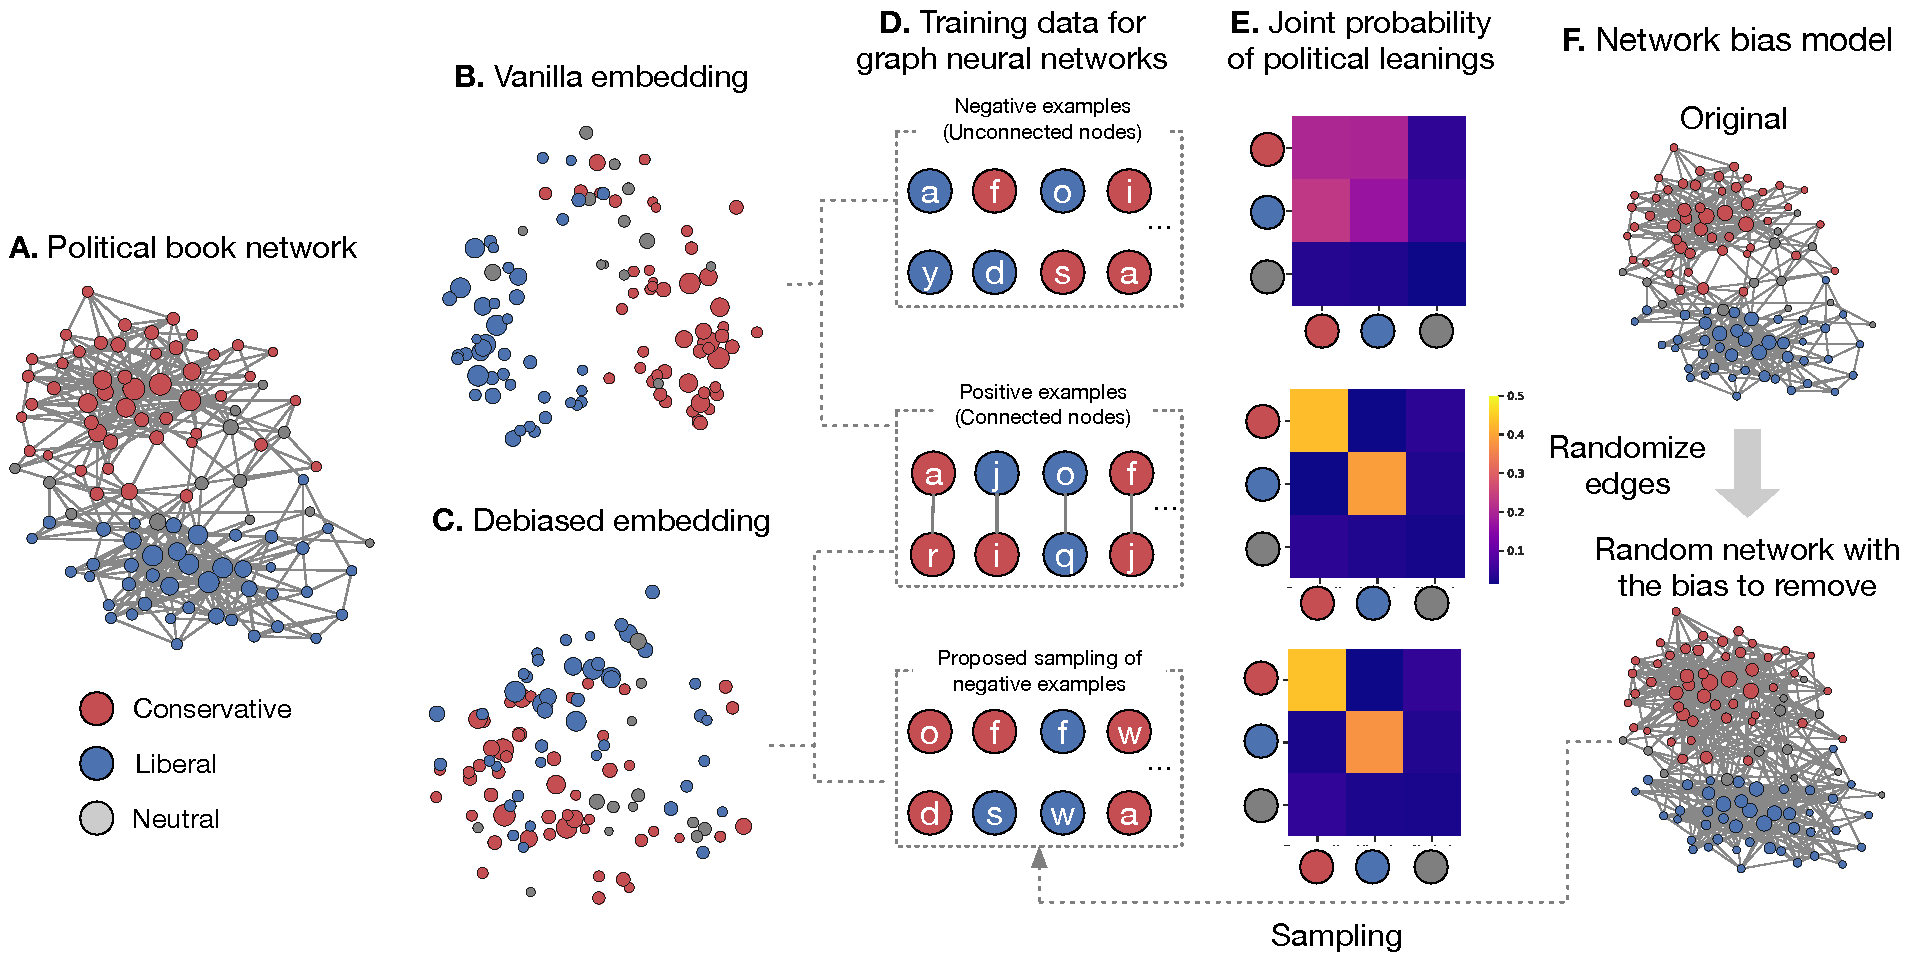
\includegraphics[width=\hsize]{images/schematics.pdf}
\caption{%
    Proposed debiasing framework. 
    {\bf A.} The political book network consists of 105 nodes representing books, with colors representing the political leaning. 
    {\bf B.} LINE graph embedding trained with a set of pairs with/without edges. 
    {\bf C.} LINE graph embedding trained with the proposed 
    debiasing framework.
    {\bf E.} Joint probability distribution of political leaning. The negative examples for vanilla LINE have no political homophily, whereas the the positive edges have a strong homophily. LINE learns this misalignment and reflected it on the embedding.
    We prevent LINE from learning the bias by aligning the political homophily, which results in the embedding with less clear political discrimination. 
    {\bf F.}  We sample the biased negative examples from a random network generated by a biased network model.  
    %This gives flexibility to the type of bias for debiasing and brings out the bias model into open. 
    %We use a biased model based on the maximum-entropy model, which randomizes the network structure while preserving the political homophily. 
    }
    \label{fig:polbook-demonstration}
\end{figure*}

Let us demonstrate a potentially harmful consequence of network biases by using a small network of political books~\cite{SocialOrganizationalNetwork}.
This network consists of $105$ books written around the time of $2004$ US presidential election consisting of $441$ edges (co-purchase relation) between books.
Many AI systems hinge on graph embedding~\cite{groverNode2vecScalableFeature2016,DBLP:journals/corr/HamiltonYL17,perozziDeepWalkOnlineLearning2014,https://doi.org/10.48550/arxiv.1710.10903}, where each node is represented as a point in space, with geometry reflecting the network structure.
The network has a strong political discrimination, and so does the embedding generated by a standard graph embedding---LINE~\cite{tangLINELargescaleInformation2015} (Fig.\ref{fig:polbook-demonstration}B).
Recommendation systems based on the embedding 
may promote books with a specific ideology and reinforce echo chambers while sidelining other viewpoints, ultimately exacerbating political polarization. 
%Thus, it is critical to ensure that the embeddings are fair and unbiased in order to mitigate these harmful consequences.

A common debiasing approach is based on the manipulation of the input data and output embedding, e.g., balancing the training data~\cite{khajehnejadCrossWalkFairnessenhancedNode2022,rahmanFairwalkFairGraph2019,solaimanProcessAdaptingLanguage2021} or removing embedding dimensions associated with bias~\cite{DBLP:journals/corr/BolukbasiCZSK16a,ravfogel-etal-2020-null}.
However, these manipulation approaches may degrade embedding quality, fail to remove the bias, or even worse, introduce a new bias~\cite{ravfogel-etal-2020-null,boseCompositionalFairnessConstraints2019,Edwards2015CensoringRW}.
An alternative approach is adversarial learning, in which  an adversarial model attempts to extract any biased features from the embedding, while the embedding is modified to be resistant to the adversary's attempts.
%In adversarial learning, one trains an embedding model and an adversarial model simultaneously~\cite{boseCompositionalFairnessConstraints2019,zhao-etal-2018-learning}.
However, the adversarial learning is often hindered by its high instability and sensitivity to hyperparameters~\cite{xing2021algorithmic}.
%As a result, there is a need for more effective approaches to addressing biases in graph data analysis that can both maintain the quality of the embeddings and address biases in the model itself.

We propose a simple yet effective framework for debiasing graph data that utilizes the inherent capacity of neural networks~\cite{kojakuResidual2VecDebiasingGraph2021}. Our key idea is to use a \textit{biased contrastive learning}, which trains a neural network to discriminate between actual data and random data. By introducing a specific bias into the random data, we ensure that sensitive attributes are not informative in the discrimination, \emph{preventing biases from entering the neural network} (Fig.~\ref{fig:polbook-demonstration}C). 
The proposed training framework can be applied to a wide range of models from simple graph embedding methods (e.g., DeepWalk and node2vec) to deep graph neural networks (e.g., GCN and GAT), offering a flexible and practical alternative to existing debiasing methods.
We test our approach by using link prediction task, demonstrating that our proposed framework substantially reduces biases while maintaining high link prediction accuracy as compared to the prevailing debiasing methods. 

%This bias in networks arises because of two primary reasons. First because of the node with a high degree can influence its neighbors (degree bias). Secondly community structure of network itself can lead to bias (group bias).

%This bias is tackled at different stages in previous attempts. Some previous works suggest that we should fix it at the level of raw data itself. However, in most cases, this bias is not trivial to be identified at that level both because of the scale and in some cases inability to identify bias at a granular level by human supervision.
%There is some research done on removing the bias in data itself. However this can be difficult both because the scale of data and the effort and time required to identify biased samples and remove them. \at{Cite paper here.}
%Some works like ~\cite{DBLP:journals/corr/BolukbasiCZSK16a} suggest that this bias can be fixed after model is trained and then debias the trained embeddings. But problem with that approach is that In this paper we propose a novel approach to tackle bias while training itself.
%\sk{place a figure here and walk through the problem.
%Two problems:
%- Degree bias
%- Political leaning
%Explains ways to address the problem.
%Explain a key idea to debias the features.
%}

% Artificial intelligence (AI) enters every walk of life---from daily shopping experience to high-stake areas such as health care and law enforcement, making critical decisions that may determine our fate.
% The increasing adoption of AI systems has created a pressing need to prevent AIs to learn inappropriate social biases.
% For instance, some biased AI systems are more likely to associate female names with family-related words than career-related words, and flag Black people as twice more likely as Whites to be at a higher risk of future crimes ~\cite{DBLP:journals/corr/BolukbasiCZSK16a,propublicamachinebias}.
% This type of systemic risk calls for an urgent need for understanding the fairness of AI and creating fair AI systems.
% 
% Biases in AIs have been active subject in fields of text and image processing because of their omnipresence and popularity. There are several works which have proposed both model (for example ~\cite{DBLP:journals/corr/abs-2107-10251}) and data based (for example ~\cite{https://doi.org/10.48550/arxiv.2208.00781}) approaches along with approaches which adjust model predictions to account for accumulated bias in models (~\cite{conf/icdm/KamiranKVG12,DBLP:journals/corr/HardtPS16}). 
% However, another prevalent data type, \textit{networks} (or \textit{graph}), have attracted substantially less attention than they deserve.
% Network data appears ubiquitously across a wide range of domains such as social networks, transportation networks, financial networks, and brains.
% Network data have been utilized by powerful machine learning models to predict technological innovations, economic recession, and epidemics.
% Although the network data has been critical in social and technological domains, little attention has been paid to the risk of social biases that may creep into machine learning applications.
% 
% Many network data are inherently biased and incomplete.
% For instance, data about social networks are often dominated by a few exceptionally popular individuals because they disproportionately appear in someone's friend list. Algorithms trained on social networks may be biased to recommend popular individuals, making them even more popular.
% In addition, humans have a strong tendency to be friends with someone with a similar demographic profile such as gender and ethnicity. Algorithms may learn the strong homophily and may influence critical human decisions which will eventually be biased. This homophily principle is a major component of almost all relationship network structures, including but not limited to work, friendship, and support groups. 
% 
% Both CrossWalk and FairWalk are recent and very popular model-free methods to debias networks' structure. The problem with both of them is that they are very generic and do not factor in the attributes of nodes. All they consider is the structure of the network to change the weights of the edges connecting different nodes in the graph. CrossWalk disproportionately weights boundary edges more than internal ones which connect nodes of other groups, as compared to Fairwalk but for both, the purpose is to facilitate the cross-connection of different groups so that it is easier for random walkers to jump from one group to another. This is a major limitation of these methods, which sometimes can result in the lowered performance of the model.
% \sk{
%   Placeholder for a related works.
%   Summarize related works starting from the debiasing approach in text and image proecssing and then graph embedding (fairwalk and cross walk).
%   Summarize what they are missing, and why it is critical.
% }

%In this paper, we introduce a generic non-parametric training framework, which results in machine learning models which are fairer which we demonstrate using link prediction metrics. Bias is an inseparable part of output models of considerable size. This bias is generally the result of the data itself on which the model is trained.
%
%Let us demonstrate the effectiveness of our approach.
%
%This image ~\ref{fig:polbook-demonstration} is obtained using PCA on generated 16-dimensional embeddings for Political Book network. As we can see nodes in the network represent clear clusters. This is the result of latent bias in the network.
%
%
%This bias in networks arises because of two primary reasons. First, the node with a high degree can influence its neighbors (degree bias). Secondly, the community structure of the network itself can lead to bias (group bias).
%
%This bias is tackled at different stages in previous attempts. Some previous works suggest that we should fix it at the level of raw data itself. However, in most cases, this bias is not trivial to be identified at that level both because of the scale and in some cases inability to identify bias at a granular level by human supervision.
%
%There is some research done on removing the bias in data itself. However, this can be difficult both because of the scale of data and the effort and time required to identify biased samples and remove them. 
%
%Some works like ~\cite{DBLP:journals/corr/BolukbasiCZSK16a} suggest that this bias can be fixed after model is trained and then debias the trained embeddings. But problem with that approach is that these methods mostly hide the bias rather than trying to remove it ~\cite{DBLP:journals/corr/abs-1903-03862}. In this paper, we propose a novel approach to tackle bias while training itself.

%\sk{place a figure here and walk through the problem.
%Two problems:
%- Degree bias
%- Political leaning
%Explains ways to address the problem.
%Explain a key idea to debias the features.
%}


\section{Method}



\subsection{Networks}

We assume that a network consists of $N$ nodes and $M$ edges. 
Each node $i$ has a $C$-dimensional vector $x_i$ representing the $i$'s attributes. Each edge $(i,j)$ between nodes $i$ and $j$ can be directed and have weight $w_{ij}$. We assume that the given network is weakly connected---every node is reachable from every other node when we ignore the direction of the edges.
%We assume that the sensitive attributes are categorical (e.g., gender) and denote by $c_i$ the sensitive attribute of node $i$.

\subsection{Link prediction}

Missing link prediction is a central task of graph representation learning and the basis of recommendation systems for social networks.  
We test graph neural networks with a standard benchmark of link prediction as follows. 
First, we randomly partition the set of edges in a given undirected network into a training set and a test set of almost an equal size while keeping the network constructed from the train edges being connected~\cite{groverNode2vecScalableFeature2016,persona2vec}.
We ensure the connectedness of the test network by adding the edges in a minimum spanning tree to the train set~\cite{groverNode2vecScalableFeature2016,persona2vec}.
Second, we generate negative edges---the pairs of unconnected nodes $(i,j)$---from the given network by sampling $i$ and $j$ uniformly at random.
We generate the same number of negative examples as the number of test edges. 
Third, we train a graph embedding model using the network constructed with the train edge set.
Fourth, for each test edge and negative edge, we calculate the likelihood of edge between two nodes by the dot similarity of the nodes' embedding vectors.
We evaluate the likelihood of edge by using the area under curve of the receiver operating characteristics curve (AUC-ROC). 
We run the experiment five times with different random seeds.

%We assess the performance of link prediction from two perspectives: disparity and accuracy. 
%We consider a link prediction is neutral with respect to the protected attributes $g$ if the predicted edges have the same distribution of $(g_i,g_j)$ with that for random predictions.
%Based on this idea, we go through each node $i$ and then 
%predict $10$ edges to other nodes having the highest prediction scores, ${\cal N}_{\text{pred}}$ ($|{\cal N}_{\text{pred}}| = 10$).
%Then, we calculate the distribution $P_{\text{pred}}(g \vert i)$ of $g$ for the predicted neighbors ${\cal N}_{\text{pred}}$.
%We define the \textit{disparity} for node $i$ by the distance between 
%the distribution and that for random prediction measured by the relative entropy 
%\begin{align}
%-\sum_{j \in {\cal N}_{\text{pred}}} P_{\text{pred}}(g_j \vert i) \log P_{\text{rand}}(g_j), \label{eq:disparity}
%\end{align}
%where $P_\text{rand}(g_j)$ is proportional to the frequency of $g_j$ for all nodes.
%A smaller score indicates stronger parity, with the minimum being zero (i.e., neutral link prediction).
%Finally, we take an average of Eq.~\eqref{eq:disparity} over all nodes as the disparity score. 
%
%In terms of prediction accuracy, a good \textit{unbiased} model can differentiate the test edges and unconnected node pairs (i.e., negative edges) \textit{without using the protected attributes}.
%Thus, we sample the negative edges such that the protected attributes are not informative in discriminating the test and negative edges. 
%Operationally, we sample a negative edge $(i,j)$ with probability
%\begin{align}
%P_n(i,j) = \frac{2M d_id_j\Lambda_{c_i,c_j}}{D_{c_i}D_{c_j}},
%\end{align}
%where $D_{c_i}$ (or $D_{c_j}$) is the sum of the degree of nodes having the same attribute $c_i$ (or $c_j$) with $i$ (or $j$), and 
%$\Lambda_{k\ell}$ is the number of edges between groups of attribute $k$ and $\ell$.
%Note that $P_n(i,j)$ produces negative edges having the same covariances of the protected attributes and the degree distribution with the positive edges, and we derive $P_n(i,j)$ based on a maximum entropy model~\cite{karrerStochasticBlockmodelsCommunity2011}  (see Appendix \ref{sec:maximum-entropy}).
%
%We sample the same number of negative edges as the test edges. 
%Then, we calculate the prediction performance by the area under curve of the receiver operating characteristic (AUC-ROC) for the prediction score for the test and negative edges.


\subsection{Key idea}

Graph neural network for link prediction is trained to differentiate the presence and absence of edges, a training framework called \textit{contrastive learning}~\cite{kojakuResidual2VecDebiasingGraph2021,dyer2014,Gutmann2010}.
Contrastive learning has been used not only for link prediction but also for a variety of tasks including natural language processing and image recognition. For example, in a face recognition task, a neural network learns a person's face $x$ by contrasting it with a reference face $x'$ of a randomly-sampled person.
The neural network recognizes target face $x$ by focusing on the \textit{differences} to the reference face $x'$.
Now, if we sample reference $x'$ from the same ethnic group as target $x$, the neural network learns the differences within the group, rather than learning ethnic traits. This can prevent the neural network from developing ethnic bias.

In context of graph embedding, a positive example is an edge $x=(i,j)$ between nodes $i$ and $j$. A negative example (or negative edge) is a pair of unconnected nodes $x'=(i',j')$ in a given network~\cite{kojakuResidual2VecDebiasingGraph2021}.
As in the case of face recognition task, a graph embedding model learns the \textit{difference} between the positive edge $x$ and negative edge $x'$. Our key idea is to generate the negative edges with the same biases so that the positive and negative edges are \texit{indistinguishable} in terms of the biases, which prevents the graph embedding model from learning the biases. 

Let us demonstrate our key idea by using the political book network.
Consider the political orientations as a sensitive attribute, and we want remove them from the embedding. 
The political attribute correlates with the network structure, namely a book is likely to be connected with the one with the same political leaning, resulting in many positive edges formed by books with the same political leaning (Fig.~\ref{fig:polbook-demonstration}E).
Now, many graph neural networks including LINE are trained on negative edges that are sampled uniformly at random.
Since the sampling of negative edges are independent of political leaning, the sampled negative edges do not have strong political homophily.
This results in the misalignment of the positive and negative edges in terms of political homophily, which is then picked up by a graph embedding model as a useful feature for discrimination.

We prevent the model from using the sensitive attribute by generating negative examples with the same bias characteristics as the positive examples.
To this end, we randomize the structure of a given network while preserving the joint probability of political leaning based on the maximum-entropy framework~(Fig.~\ref{fig:polbook-demonstration}F; see the Model of network bias section). 
This results in a random network that is indistinguishable from the given network in terms of the political assortativity (Fig.~\ref{fig:polbook-demonstration}E), and the resulting graph embedding has no visible political separation accordingly (Fig.~\ref{fig:polbook-demonstration}C).
%In what follows, we show that this bias sampling of negative edges prevent biases from entering the graph embedding.  
%
%
%For the political book network, our biased contrastive learning is effective in removing political separations in DeepWalk, whereas an existing debiasing method, Crosswalk, fails (Fig.\ref{fig:polbook-demonstration}D). 
%Our approach can be applied to more complex models such as the Graph Attention Network (GAT)~\cite{https://doi.org/10.48550/arxiv.1710.10903} and still produce similar results.

\subsection{Contrastive learning for debiasing}

We focus on graph neural networks that generate a node embedding based on the network structure and node features. 
We express a graph neural network as a function $\phi$ parameterized by $\vec{\theta}$ that produces an embedding of node $i$, i.e., $\phi(i;\vec{\theta}) \in {\mathbb R}^{K\times 1}$.
In link prediction, a graph neural network learns the probability $P(i,j)$ that an edge appears between two nodes $(i,j)$, a common form being the softmax function, i.e.,  
\begin{align}
    P(i,j) = \frac{1}{Z} \exp(\phi(i)^\top \phi(j)).
    \label{eq:graph_neural_net}
\end{align}
Variable $Z$ is a normalization constant. Fitting the softmax function is notoriously difficult since $Z$ is computationally demanding as it extends over all node pairs. Thus, several efficient estimation methods have been developed.

Noise contrastive learning (NCE) is an efficient estimation method for Eq.~\eqref{eq:graph_neural_net}~\cite{Gutmann2010}. 
The key idea underlying NCE is to train a different computationally-cheaper model whose best parameter $\theta^*$ in terms of the likelihood being the same as Eq.~\eqref{eq:graph_neural_net}.
Operationally, NCE trains a logistic regression model by classifying a set of node pairs $(i,j)$ into \textit{connected} node pairs and randomly-sampled node pairs, i.e.,  
\begin{align}
P\left(Y_{ij} = 1\right):= \frac{1}{1 + \exp(-f(i,j) + \ln P_0(i,j))},
\label{eq:nce}
\end{align}
where $Y_{ij} = 1$ if nodes $i$ and $j$ are connected, $Y_{ij}=0$ if they are not, and $f(i,j)=\phi(i) ^\top \phi(j)$ is the node similarity. 
It is shown that NCE is asymptotically unbiased for an exponential probability model given by~\cite{Gutmann2010,dyer2014}:
\begin{align}
P(i,j) = \frac{1}{Z}\exp(f(i,j)), \label{eq:exp_func}
\end{align}
which corresponds to the edge probability learned by a graph neural network given inEq.~\eqref{eq:graph_neural_net}.

A key feature of NCE is that it is unbiased estimator agnostic to the choice of $P_0(i,j)$ because the effect of $P_0(i,j)$ is offset by $\ln P_0(i,j)$ in Eq.~\eqref{eq:nce}. Removing the offset gives rise to a powerful capacity of debiasing, as is demonstratd by \cite{kojakuResidual2VecDebiasingGraph2021}.
Let us consider NCE without the offset $\ln P_0(i,j)$, i.e., discriminating the connected and unconnected node pairs by  
\begin{align}
P\left(Y_{ij} = 1\right):= \frac{1}{1 + \exp(-\phi(i) ^\top \phi(j))} 
\label{eq:nce_simplified}
\end{align}
Because we drop $\ln P_0(i,j)$, Eq.~\eqref{eq:nce_simplified} gives a biased estimate.
To see the effec of the bias, we derive a model for which Eq.~\ref{eq:nce_simplified} is unbiased for by rewriting  Eq.~\eqref{eq:nce_simplified} in form of NCE as 
\begin{align}
P\left(Y_{ij} = 1\right) &:= \frac{1}{1 + \exp\left(-f'(i,j)+ \ln P_0(i,j)\right]}
\label{eq:nce_simplified2}
\end{align}
where $f(i,j):=\phi(i) ^\top \phi(j) + \ln P_0(i,j)$. Since Eq.~\eqref{eq:nce} is unbiased estimator for Eq.~\eqref{eq:exp_func}, Eq.~\eqref{eq:nce_simplified2} is asymptomatically unbiased for 
\begin{align}
P(i,j) &= \frac{1}{Z'}\exp(f'(i,j)) \nonumber \\
       &= \frac{1}{Z'}P_0(i,j)\exp(\phi(i) ^\top \phi(j)).
\label{eq:residual2vec}
\end{align}
Equation~\eqref{eq:residual2vec} decomposes the probability of edge $P(i,j)$ into $P_0(i,j)$ and node similarity $\phi(i) ^\top \phi(j)$. From a different perspective, noise distribution $P_0(i,j)$ serves as a \textit{null model} for networks, accounting for trivial relationships of nodes. The node similarity captures the \textit{residuals} from $P_0(i,j)$, reflecting the non-trivial relationships not explained by the null model.
This insight enables us to debias graph embedding, i.e., by introducing a bias into the null model, we can in turn remove the bias in the residual, from which the embedding is constructed. 

The advantage of our approach is that the bias model is clear and explicit. 
All debiasing methods assume some null models because they must make judgment about when two nodes should be closer to each other than others.
However, the assumptions are often unclear, even when the algorithm itself is simple. 
By making clear the bias model, we gain greater control over the process of debiasing and a deeper understanding of its consequences. 

\subsection{Models of network bias}

The bias model should exhibit the same type and extent of bias while having no other structure.
We construct such a bias model based on the maximum entropy principle~\cite{cimini2019statistical,bardoscia2021physics}.
Specifically, we want the noise distribution $P_0(i,j)$ to be maximally random, i.e., maximizing the entropy  
\begin{align}
-\sum_{i,j} P_0(i,j) \log P_0(i,j),
\end{align}
while preserving the assortativity over the protected groups:
\begin{align}
\sum_{i \in {\cal C}_\ell}\sum_{i \in {\cal C}_k} P_0(i,j) &= \sum_{i \in {\cal C}_\ell}\sum_{i \in {\cal C}_k}P(i,j),
\end{align}
for all $1 \leq k, \ell \leq L$, where $L$ is the number of unique protected groups, and ${\cal C}_k$ is the set of nodes in the $k$th group. 
Finding the $P_0(i,j)$ is a constrained optimization problem, which can be formulated as a Lagrangian:
\begin{align}
{\cal L}:&= -\sum_{i,j} P_0(i,j) \log P_0(i,j) \nonumber \\
&+ \sum_{k=1}^L\sum_{\ell=k}^L \beta_{k\ell}
\left( 
\sum_{i \in {\cal C}_\ell}\sum_{i \in {\cal C}_k} P_0(i,j) - \sum_{i \in {\cal C}_\ell}\sum_{i \in {\cal C}_k}P(i,j) \right).
\end{align}
By taking a functional derivative with respect to $P_0$ and solving 
$\partial {\cal L}/\partial P_0$ = 0, we obtain
\begin{align}
P_0(i,j) &= \text{Poisson}(\lambda_{ij}), \\
\lambda_{ij} &= \frac{1}{|{\cal C}_{c_i}||{\cal C}_{c_j}|}\sum_{i \in {\cal C}_\ell}\sum_{j \in {\cal C}_k} P(i,j).
\end{align}
This bias model is maximally random while preserving the same type and extent of bias in the given network. 
One can have additional constraints to model a more complex network bias, i.e., degree heterogeneity, degree-degree correlation, and edge directionality. 
See \cite{cimini2019statistical,bardoscia2021physics} for other network models based on the maximum entropy principle. 



%\subsection{Debiasing graph neural networks for link prediction}
%We train the GNN by using a biased contrastive learning, where the positive examples are sampled from in a given network, and the negative edges are sampled from random networks. 
%We use the degree-corrected stochastic block model (dcSBM) to generate random networks. Each block in the dcSBM corresponds to a group of nodes that share the same sensitive attributes. The dcSBM preserves the number of edges between and within each group, resulting in negative edges having the same covariance of protected attributes as positive edges.
%The dcSBM is used by residual2vec~\cite{kojakuResidual2VecDebiasingGraph2021}, which is a special case of the GNNs that trains node2vec~\cite{grover_node2vec_2016} with a biased contrastive learning.  
%While node2vec uses separate encoders for each node in a pair to learn the asymmetric relationships between them. 
%However, in the case of undirected networks, relationships are symmetric, and thus, using a single encoder for both nodes produce similar representation~\cite{qiuNetworkEmbeddingMatrix2018,kojakuResidual2VecDebiasingGraph2021}.
%
%Let us showcase the proposed method by using the political book network (Fig.\ref{fig:polbook-demonstration}),
%DeepWalk, GCN, and GAT trained with the biased contrastive learning do not show a clear political separation in the embeddings, despite their differences in the architecture and training objectives. This result demonstrates the systematic effectiveness of the biased contrastive learning method in debiasing.
%
%\subsubsection{Debiasing for graph representation learning}
%
%Many graph representation is generated based on node triplets $(i,j,j')$ encoding local structure around each node $i$; node $j$ represents a context randomly sampled from the neighborhood of node $i$, where the neighborhood refers to direct neighbors neighbors~\cite{tangLINELargescaleInformation2015} or nodes with close proximity~\cite{perozziDeepWalkOnlineLearning2014,groverNode2vecScalableFeature2016}. Node $j'$ represents a \textit{random} context sampled from a random distribution $P_0(j')$.
%One generates a graph embedding by discriminating actual context $j$ and random context $j'$ by using a logistic function:
%\begin{align}
%\frac{1}{1 + \exp(-u_i ^\top v_j)},
%\end{align}
%where $u_i$ and $v_i$ are the in-vector and out-vector that represent a node $i$ as an anchor and context node respectively.
%This training process is negative sampling, and thus, learns probability model
%\begin{align}
%P(j \vert i) = \frac{1}{Z'}P_0(j)\exp\left(u_i ^\top v_j\right), \label{eq:graph_representation_model}
%\end{align}
%where $P(j\vert i)$ is the probability that $j$ is sampled from the neighborhood of $i$, representing a structural association between nodes $i$ and $j$. Equation~\ref{eq:graph_representation_model} decomposes the structural association into $P_0(j)$ and $\exp\left(u_i ^\top v_j\right)$, where $P_0(j)$ plays a role as a \textit{baseline} probability, and embedding vectors $u_i$ and $v_j$ encode \textit{residual} not explained by the baseline.
%residual2vec utilizes this implicit decomposition for debiasing a shallow neural network---word2vec---for graph representation learning~\cite{kojakuResidual2VecDebiasingGraph2021}.
%The key idea is to explicitly model $P_0$ that accounts for the structural associations attributed to a focal bias and train embedding on the residual unbiased component.
%For instance, for a social network with strong gender homophily, one can generate a gender-neutral embedding by using a biased baseline $P_0$ that samples a random context node $j'$ whose distribution is statistically indistinguishable with actual context $j$ with respect to gender. Since both contexts $j$ and $j'$ are indistinguishable by gender, embedding---which is trained to distinguish $j$ and $j'$ by negative sampling---learns something other than gender.
%


% \begin{figure*}[t!]
%     \centering
%     \begin{subfigure}[t]{0.5\textwidth}
%         \centering
%         \includegraphics[width=2in]{images/demonstration/dw.png}
%     \end{subfigure}
% \hfill

%     \begin{subfigure}[t]{0.5\textwidth}
%         \centering
%         \includegraphics[width=2in]{images/demonstration/dw.png}
%     \end{subfigure}


% \end{figure*}

%Let us demonstrate the effectiveness of our approach using a small toy network, namely political book network.
%We train the Graph Attention Network (GAT) and use the DeepWalk to generate node features for respective nodes.
%The GAT without debiasing discriminates the books of different political leaning, reflecting the fact
%that books supporting the same political belief are likely to be bought together (Fig.~\ref{fig:demonstration_gat_random}).
%The use of embedding in a recommendation system may create a filter bubble, in which users are presented with a biased selection of books based on their initial political beliefs.
%
%To break filter bubble, it is necessary to create an embedding that does not discriminate books based on their political leaning.
%To this end, we employed a biased sampling of negative sampling that accounts for structural biases pertained to a categorical variable (i.e., political learning in our toy example)~\cite{kojakuResidual2VecDebiasingGraph2021}.

\section{Results}

\subsection{Datasets}

\begin{table*}
\centering
  \caption{
    Statistics of network data for link prediction.
    Information modularity indicates the strength of the communities in a network, where each community is a set of nodes with the same protected attribute. See \ref{}\sk{add the robustness modularity paper}.  
  }
  \label{table:datasets}
  \begin{tabular}{lllp{10em}p{10em}}
  \toprule
        \multirow{2}{*}{Network} & \multirow{2}{*}{Nodes} & \multirow{2}{*}{Edges} & Protected category & \multirow{2}{*}{Information Modularity}\\
        & & &  (\# of categories) & \\ 
    \midrule
Political Books & \num{105} & \num{441} & Political leaning (3) & \num{0.061}\\
Political Blogs & \num{1224} & \num{16715}  & Political leaning  (3) & \num{0.0925}\\
Airport & \num{2898} & \num{15564}  & Geographical regions (5) & \num{0.112}\\
    Twitch       & \num{168114} & \num{6797557}  & Language (20) & \num{0.05}\\
    
    Facebook       & \num{41554} & \num{1362229}  & Gender (3) & \num{-0.004}\\
    \bottomrule
  \end{tabular}
\end{table*}

We test GNNs with four different networks (Table\ref{table:datasets}):
the political books~\cite{nr}, the political blogs~\cite{10.1145/1134271.1134277}, the airport network~\cite{OpenFlig19:online}, twitch gamers  ~\cite{rozemberczki2021twitch} and Facebook network ~\cite{DBLP:journals/corr/abs-1102-2166}.
These networks include categorical attributes for nodes that we do not want to use to make link prediction (i.e., protected attributes).
For all networks, we ignore the edge directionality.

The political blog network represents the political blogs about the 2004 US presidential election connected by hyperlinks.
We use the political affiliation assigned to the blogs as the protected attribute.

The airport network is the network of airports connected by edges indicating direct commercial flight. 
We use the geographical region of the airports as the protected attribute.

Twitch dataset is a social network of Twitch gamers which was collected using public Twitch API. Graph represents a single strongly connected component and edges are the mutual follower relationships between them. We have few features as the metadata for nodes, but for this paper we used language as the protected attribute.

Facebook dataset used here is a friendship network of $100$ american colleges and universities. We use gender as a protected attribute. Nodes for which gender is unknown are given a separate group.

% The pokec network is a on-line social network in Slovakia and Czech Republic constructed from a snapshot in 2012.
% We only use the gender of each node as a protected attribute. 


%
%This method is independent of the model or features used to encode network nodes. 
%In this case, we show word2vec, GAT and GCN along with different feature generation mechanisms (DeepWalk and node2vec). 
%For smaller networks (Airport, Political Blogs and Political Book) we use 4 layers for GCNConv or GATConv stacked over one another while for Pokec we use 5 followed by 2 linear layers.

\subsection{Graph neural network models}

We test three graph neural networks with different architectures: word2vec (a neural network with one hidden linear layer and the softmax output layer)~\cite{mikolovDistributedRepresentationsWords2013}, GCN ~\cite{kipf2017semisupervised}, and GAT ~\cite{velickovicGraphAttentionNetworks2022}.
The GCN and GNN needs node features as input, for which we 
use $K=128$ dimensional embedding vectors generated by DeepWalk.
We find that using node2vec instead of DeepWalk yield qualitatively the same results (Appendix).
To see the effect of debiasing, we compare each model trained with the proposed bias sampling of negative examples with the one with with a conventional uniform sampling.
We also employ two families of debiasing methods as baselines. 
One family is based on the manipulating network data to balance the training data for DeepWalk, i.e., FairWalk~\cite{rahmanFairwalkFairGraph2019} and CrossWalk~\cite{khajehnejadCrossWalkFairnessenhancedNode2022}.
The other family is based on the manipulation of the output embedding, for which we use a debiasing method based on linear projection ~\cite{DBLP:journals/corr/BolukbasiCZSK16a}. 
For a stable baseline we use the method proposed in ~\cite{DBLP:journals/corr/BolukbasiCZSK16a}. To apply this method to a graph, we use PCA to determine the bias direction using $20\%$ of the nodes nearest to group centroids. As opposed to the previous work we do not have any gender neutral nodes. We use all the nodes as equalize nodes. We change embedding of each node as
\begin{align}
\overrightarrow{W} := \overrightarrow{W} - \overrightarrow{D} \cdot \textit{proj}_{\overrightarrow{W}}\overrightarrow{D}
\end{align}

where $\overrightarrow{D}$ is the bias direction.
\subsection{Bias in graph embedding}

We quantify the biases in graph embedding by the extent to which the sensitive attribute shapes the structure of the embedding.
If we were to have an well-debiased graph embedding, the sensitive attributes should not be the main dimensions of the graph embedding.  
Following the previous study~\cite{DBLP:journals/corr/BolukbasiCZSK16a}, we identify the embedding dimensions that are the most coherent to sensitive attributes and then quantify the ratio of explained variance to total variance of the nodes in the embedding as the level of bias (Fig.~\ref{fig:xxx}).
We find that ...

While the sensitive attributes may not entirely shape the embedding structure, they could still have a local impact on the proximity of nodes. 
To examine the impact on the local proximity, we test to what extent each node is equidistance to the protected groups. More specifically, for each node $i$ with embedding vector $\vec{u}_{i}$, we compute the cosine similarity (i.e., $\cos(\vec{u}_i, \vec{u}_\ell)$) to the centroid vector $\vec{u}_\ell$ of each group $c=\ell$. Then, we compute the \textit{local disparity} $D_i$ by the variance over all groups, i.e., 
\begin{align}
D_i:= \frac{1}{L}\sum_{\ell=1}^L \left(\cos(\vec{u}_i, \vec{u}_\ell) - \frac{1}{L}\sum_{\ell'=1}^L \cos(\vec{u}_i, \vec{u}_{\ell'})\right)^2.
\end{align}
We find that the local disparity drops for majority of nodes in the network when trained using biased negative sampling (Fig.~\ref{fig:}). The reduction of disparity is overall consistent across different model architecture and networks.  

In summary, our training framework consistently brings a reduction of biases in graph neural networks compred to their unbiased counterparts across different networks both at global and local levels. The reduction of bias is comparable or substantial compared to the baseline debiasing methods. These results demonstrate that our training framework for debiasing is consistently effective and model-independent in reducing the biases in graph embedding.  

\subsection{Prediction performance}

Debiasing an embedding involves masking certain information within the embedding, which can potentially lead to a significant reduction in the embedding's utility.
Indeed, the debiasing methods including our method and the baselines all results in the decreased link prediction performance. However, the amount of the decrease differs method by methods. In fact, our training method results in the least decreases in the performance among all the debiasing methods (Fig.~xxx). 

We also examine the utility of embedding at a local node. 
For each node, we find the 50 closest neighbors in the given embedding. Then, we calculate the average precision of the node similarity for the test edges. 
xxxx



%We also see a significant drop in cumulative disparity for all the nodes in the network when trained using biased negative sampling \ref{sec:maximum-entropy} versus negative nodes sampled randomly. 
%Fig. \ref{fig:disparity_per_node_deepwalk} captures the same disparity. This figure plots the ratio of nodes for which cumulative disparity score decreased vs increased. This disparity is the standard deviation of cosine similarity of a node with centroids of every protected group. This plot summarizes the results for different model architectures(rows) and datasets(columns) and results indicate that in almost every case, the number of nodes having larger disparities decreases by a significant margin and thus improves the recommendation results. \emph{Disparity} is defined here as
%\begin{align}
% \frac{1}{|G|}\sum_{i \in G} \sum_{j \in G} \left| \frac{1}{|G|}\sum_{k \in G} \cos(\mathbf{v}_i, \mathbf{v}_k) - \frac{1}{|G|}\sum_{k \in G} \cos(\mathbf{v}_j, \mathbf{v}_k) \right|
%\end{align}
%where $G$ is the set of protected groups in the graph, $\mathbf{v}_i$ is the embedding of node $i$ and $\cos(\mathbf{v}_i, \mathbf{v}_j)$ is the cosine similarity between the embeddings of nodes $i$ and $j$.
%
%
%We notice that in almost all cases the number of nodes for which this disparity increases is smaller than for the number of nodes for which it decreases (disparity score $\geq$ .5). This indicates that the proposed method decreases the overall disparity in the network. This results in better recommendations on average for all nodes.
%
%
%\subsection{Prediction performance}

%We evaluate the performance of these models using two link prediction metrics: AUC-ROC and Statistical Parity.
%Results are demonstrated in figures \ref{fig:roc} and \ref{fig:sp} respectively. In both of these figure we compare our training method with Crosswalk, Fairwalk, Deepwalk. We also include plots for GNNs which can be used to compare our sampling method with similar models when trained with uniformly randomly sampled negative neighbors.
%To calculate statistical parity, we pick the $5$ nearest neighbors using cosine distance on the $128$ dimensional embeddings. We then create a graph using those edges and then calculate statistical parity on that network. \at{explain statistical parity here}

\begin{figure*}[h]
\centering

        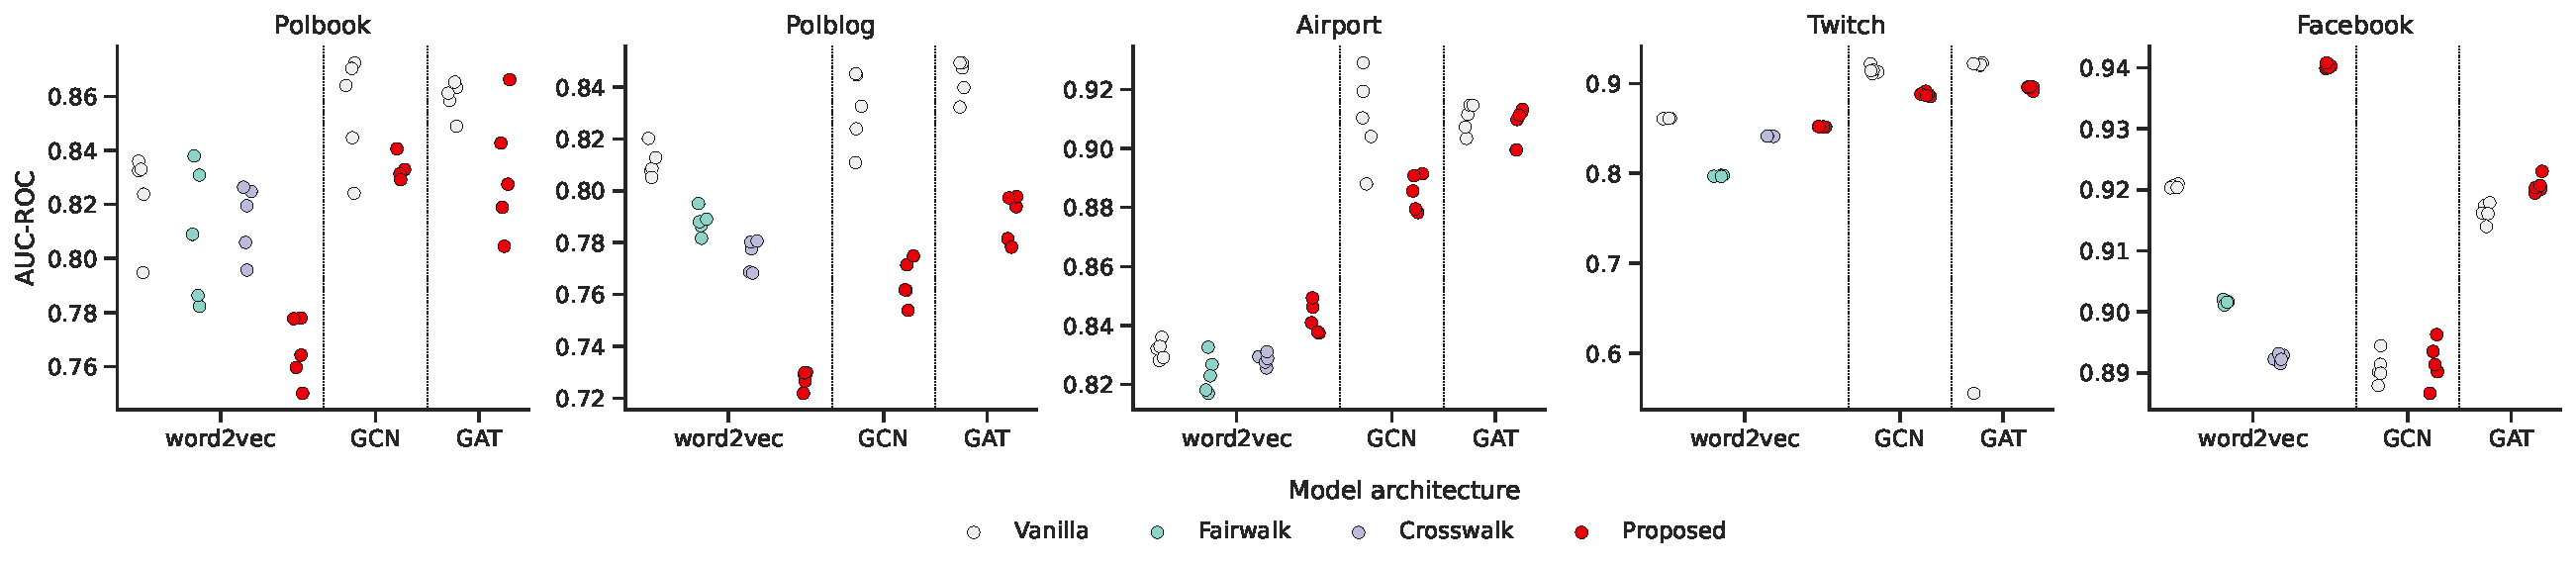
\includegraphics{images/new_images/aucroc_deepwalk_proposed_comparison.pdf}
        \label{fig:aucroc_deepwalk_manipulation_comparison}
    \caption{Link Prediction benchmark results for different datasets. Fig \ref{fig:aucroc_deepwalk} (A-E) shows the AUC-ROC scores for which negative edges were generated using \ref{sec:maximum-entropy}. Fig \ref{fig:disparity_deepwalk} (F-H) shows the disparity scores. Disparity here is defined by how invariant the model is with respect to the protected attribute in predicting the edges for test network.} 
  \label{fig:sp}
\end{figure*}

\begin{figure*}[h!]
    \centering
    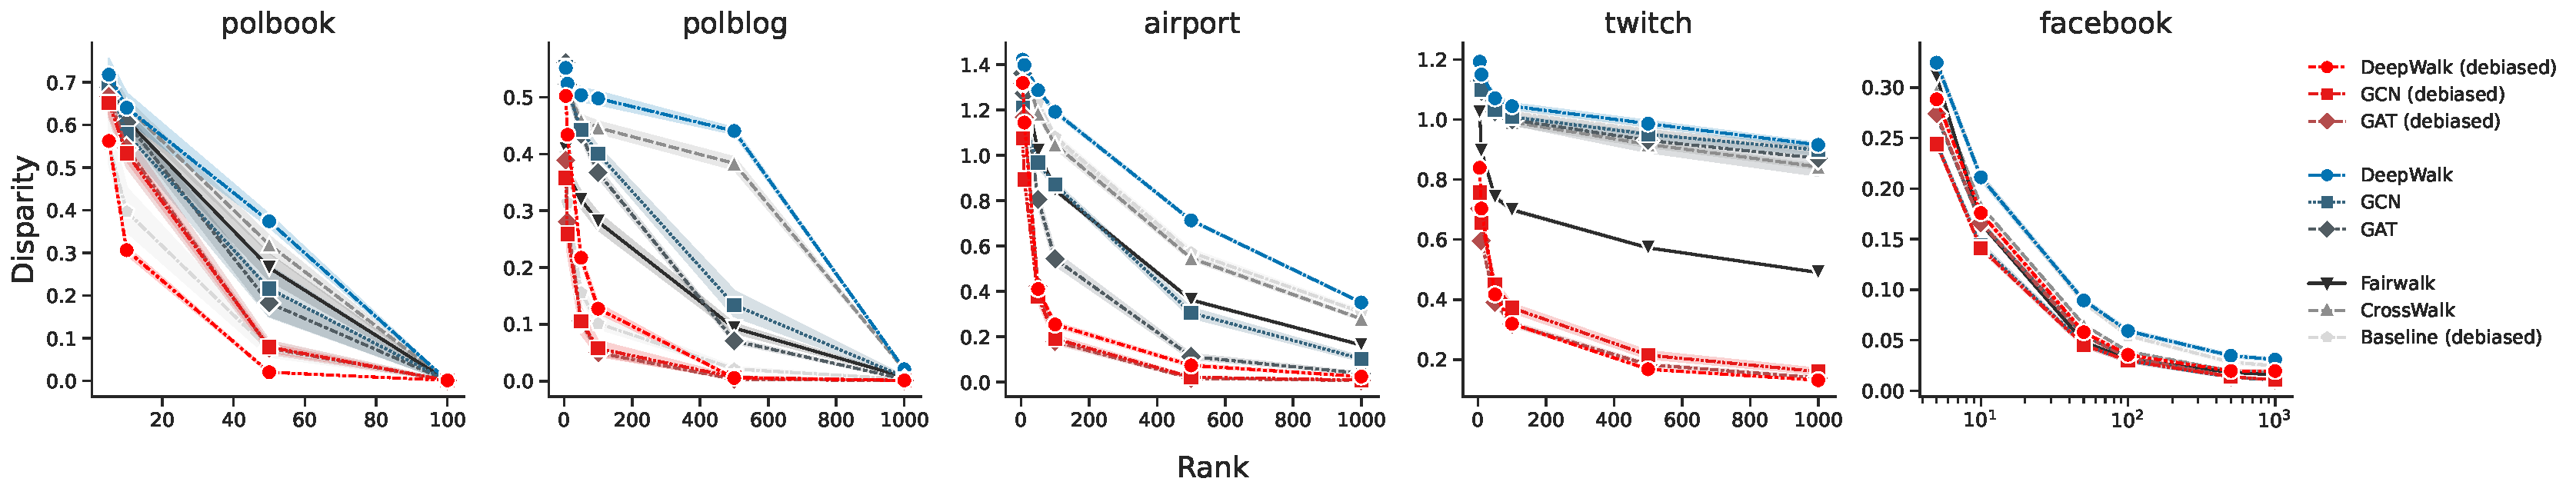
\includegraphics[width=\hsize]{images/new_images/disparity-curve_deepwalk.pdf}
    \caption{Relative Entropy of predictive group membership distribution and original group membership distribution vs k (number of nearest neighbors)}
    \label{fig:entropy_deepwalk}
\end{figure*}



\begin{figure}[h!]
    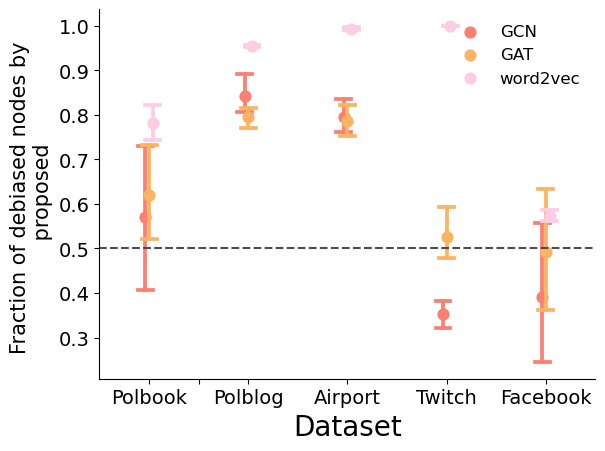
\includegraphics[width=.5\textwidth, height=.5\textwidth]{images/new_images/deepwalk_disparity_per_node.png}
    \caption{Disparity per Node, this plot demonstrates ratio of nodes for which the standard deviation of cosine similarity from the centroid of all protected groups decreased in proposed versus compared to baseline models. We see a noticeable drop in the cumulative disparity of the set of nodes. Baselines are the models trained with randomly Sampled negative nodes while proposed models are trained using proposed biased negative sampling. \at{Currently plotting just one run, should we plot average?}}
    \label{fig:disparity_per_node_deepwalk}
\end{figure}
\begin{figure}
    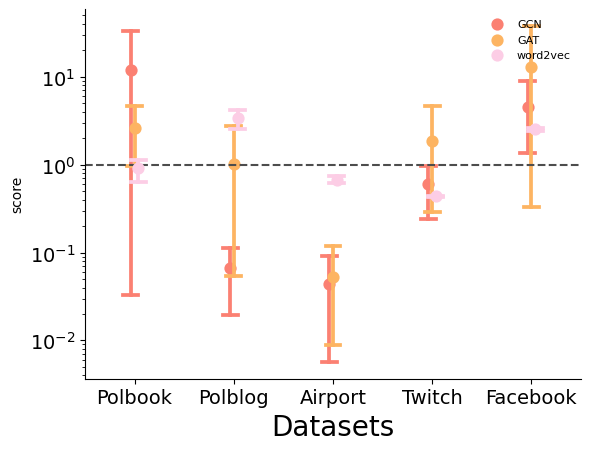
\includegraphics[width=.5\textwidth, height=.5\textwidth]{images/new_images/deepwalk_disparity_per_node_global.png}
    \caption{Global Fairness}
    \label{fig:disparity_global_deepwalk}
\end{figure}

%The debiased DeepWalk trained with the biased contrastive learning yields a better prediction performance for all networks.  
%The debiased GCN and GAT also yield a better or comparative prediction accuracy with the vannila models, suggesting that the biased contrastive learning does not negatively impact on the GNNs.
%Fairwalk and CrossWalk, which debias DeepWalk by manipulating the input network, yield comparable prediction performance as the vannila DeepWalk. 
%
%We find stark differences in the learned embedding in terms of the disparity (Figs.\ref{fig:sp}xxx).
%The use of biased contrastive learning led to a substantial reduction in the disparity score for DeepWalk in 11 out of 12 combinations of models and networks, resulting in a debiased DeepWalk with a lower disparity score than Fairwalk and Crosswalk.
%
%How is it possible to maintain the prediction accuracy while reducing the biases?
%To understand this, we vary the number $k$ of predicted edges per node for which the disparity score is calculated  (Fig.\ref{fig:entropy_deepwalk}).
%We find that the top few nodes ($k<5$) are not impacted by the biased contrastive learning, having a comparable disparity score with the vannila models.
%However, as $k$ increases, the biased contrastive learning yields a substantial reduction of the disparity score by a large margin.
%These results indicate that the biased contrastive learning respects the training objective while reducing biases in the models. 
%Consequently, the top recommendations exhibit a similar level of biases, while lower-ranked recommendations are less affected by protected attributes, compensating for the biased recommendations.
%

%Fig.~\ref{fig:entropy_deepwalk} demonstrates the disparity vs k (number of nearest neighbors). Disparity here is defined as the KL divergence between the predictive group membership distribution and the original group membership distribution. 
%Predictive group distribution is obtained here using cosine distance between the nodes as the similarity metric ~\ref{eq:disparity}.
%We observe that the entropy of the predictive group membership distribution decreases with the proposed method. This is because the proposed method reduces the disparity in the embedding space, which in turn reduces the entropy of the predictive group membership distribution. 
%
%
%Overall, our training framework consistently reduces the biases in embedding across different architecture of GNNs, making the models agnostic to the protected group attributes.  We see that in almost all cases AUC-ROC score (Fig.~\ref{fig:sp} A--D) improves with our proposed sampling method. This AUC-ROC score is obtained using the test edges and the negative edges sampled using our proposed sampling method ~\ref{sec:maximum-entropy}.
%
% \yy{I feel like we should dig into the results more}


\section{Conclusion}

We proposed a novel training framework to jointly improve fairness and quality of graph embeddings. 
We validated the proposed framework by training three models ranging from a shallow to deep neural networks.
Notably, our approach makes the biased structural features inconseqential to model training, rather than 
heuristically removing biased input data or biased dimensions in the generated embedding.
Overall, our proposed framework presents a new way to address the issue of biases in graph data, and can be applied to a variety of downstream AI applications.

There are certain limitations to be acknowledged.
First, our approach requires a biased model encoding biased associations.
We used the degree-corrected stochastic block model as the biased model by following the previous study~\cite{kojakuResidual2VecDebiasingGraph2021}.
Learning a suitable biased model for debiasing warrants future work.
Second, our approach assumes that the sensitive attribute is known and labeled, which may not always be the case in real-world scenarios. 
Third, while we have focused on direct associations between sensitive attributes, our approach may not completely eliminate bias due to indirect associations of biased attributes through other attributes~\cite{DBLP:journals/corr/abs-1903-03862}. Despite these limitations, our study demonstrates that by biasing the sampling of negative examples, it is possible to reduce bias while maintaining high accuracy in graph embedding.




% \section*{Software and Data}

% If a paper is accepted, we strongly encourage the publication of software and data with the
% camera-ready version of the paper whenever appropriate. This can be
% done by including a URL in the camera-ready copy. However, \textbf{do not}
% include URLs that reveal your institution or identity in your
% submission for review. Instead, provide an anonymous URL or upload
% the material as ``Supplementary Material'' into the CMT reviewing
% system. Note that reviewers are not required to look at this material
% when writing their review.

% Acknowledgements should only appear in the accepted version.
% \section*{Acknowledgements}

% \textbf{Do not} include acknowledgements in the initial version of
% the paper submitted for blind review.

% If a paper is accepted, the final camera-ready version can (and
% probably should) include acknowledgements. In this case, please
% place such acknowledgements in an unnumbered section at the
% end of the paper. Typically, this will include thanks to reviewers
% who gave useful comments, to colleagues who contributed to the ideas,
% and to funding agencies and corporate sponsors that provided financial
% support.


% In the unusual situation where you want a paper to appear in the
% references without citing it in the main text, use \nocite
% \nocite{langley00}

\bibliography{main}
\bibliographystyle{icml2023}


%%%%%%%%%%%%%%%%%%%%%%%%%%%%%%%%%%%%%%%%%%%%%%%%%%%%%%%%%%%%%%%%%%%%%%%%%%%%%%%
%%%%%%%%%%%%%%%%%%%%%%%%%%%%%%%%%%%%%%%%%%%%%%%%%%%%%%%%%%%%%%%%%%%%%%%%%%%%%%%
% APPENDIX
%%%%%%%%%%%%%%%%%%%%%%%%%%%%%%%%%%%%%%%%%%%%%%%%%%%%%%%%%%%%%%%%%%%%%%%%%%%%%%%
%%%%%%%%%%%%%%%%%%%%%%%%%%%%%%%%%%%%%%%%%%%%%%%%%%%%%%%%%%%%%%%%%%%%%%%%%%%%%%%
\newpage
\appendix
\onecolumn
\section{Appendix}

\subsection{node2vec with FairGraph}

Apart from trying our method with DeepWalk, we also tried it with node2vec. In this section we demonstrate that both of our contributions, FairGraph and Biased NCE Sampling work with any model and feature generation method. 

\begin{figure*}[t!]
\captionsetup[subfigure]{labelformat=empty}
    \centering
    \subfloat[(A) GAT]{%
\label{fig:demonstration_gat_random_n2v}%
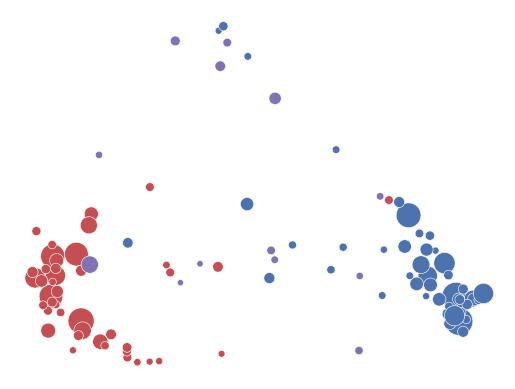
\includegraphics[scale=.5]{images/appendix/node2vec/demonstration/gat_random.png}}%
\qquad
\subfloat[(B) GAT + Biased Sampling (proposed)]{%
\label{fig:demonstration_gat_r2v_n2v}%
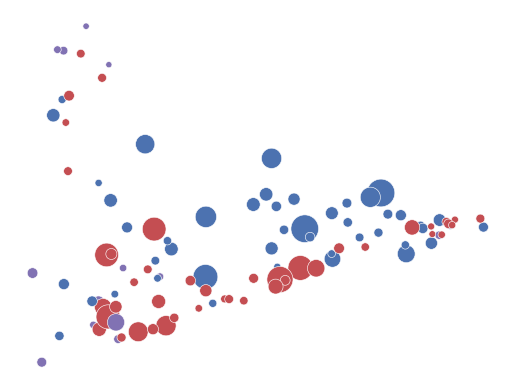
\includegraphics[scale=.5]{images/appendix/node2vec/demonstration/gat_r2v.png}}

\subfloat[(C) GCN]{%
\label{fig:demonstration_gcn_random_n2v}%
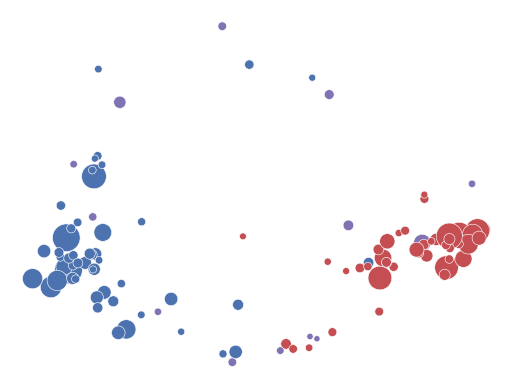
\includegraphics[scale=.5]{images/appendix/node2vec/demonstration/gcn_random.png}}%
\qquad
\subfloat[(D) GCN + Biased Sampling (proposed)]{%
\label{fig:demonstration_gcn_r2v_n2v}%
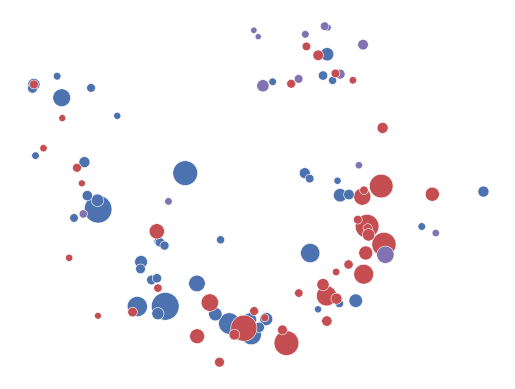
\includegraphics[scale=.5]{images/appendix/node2vec/demonstration/gcn_r2v.png}}%


    \caption{Demonstration on Political Book Dataset. Each node represents a book. The color of the node indicates the political alignment of the book, blue for liberal, red for conservative, and purple for neutral. The size of each node is proportional to the degree of a node in the original network. Images are generated using PCA on $16$ dimensional embeddings. In each of these case nodes are represented by their $16$ dimensional node2vec features}
    \label{fig:polbook-demonstration-appendix}
\end{figure*}



\begin{figure*}[h!]
    \centering
    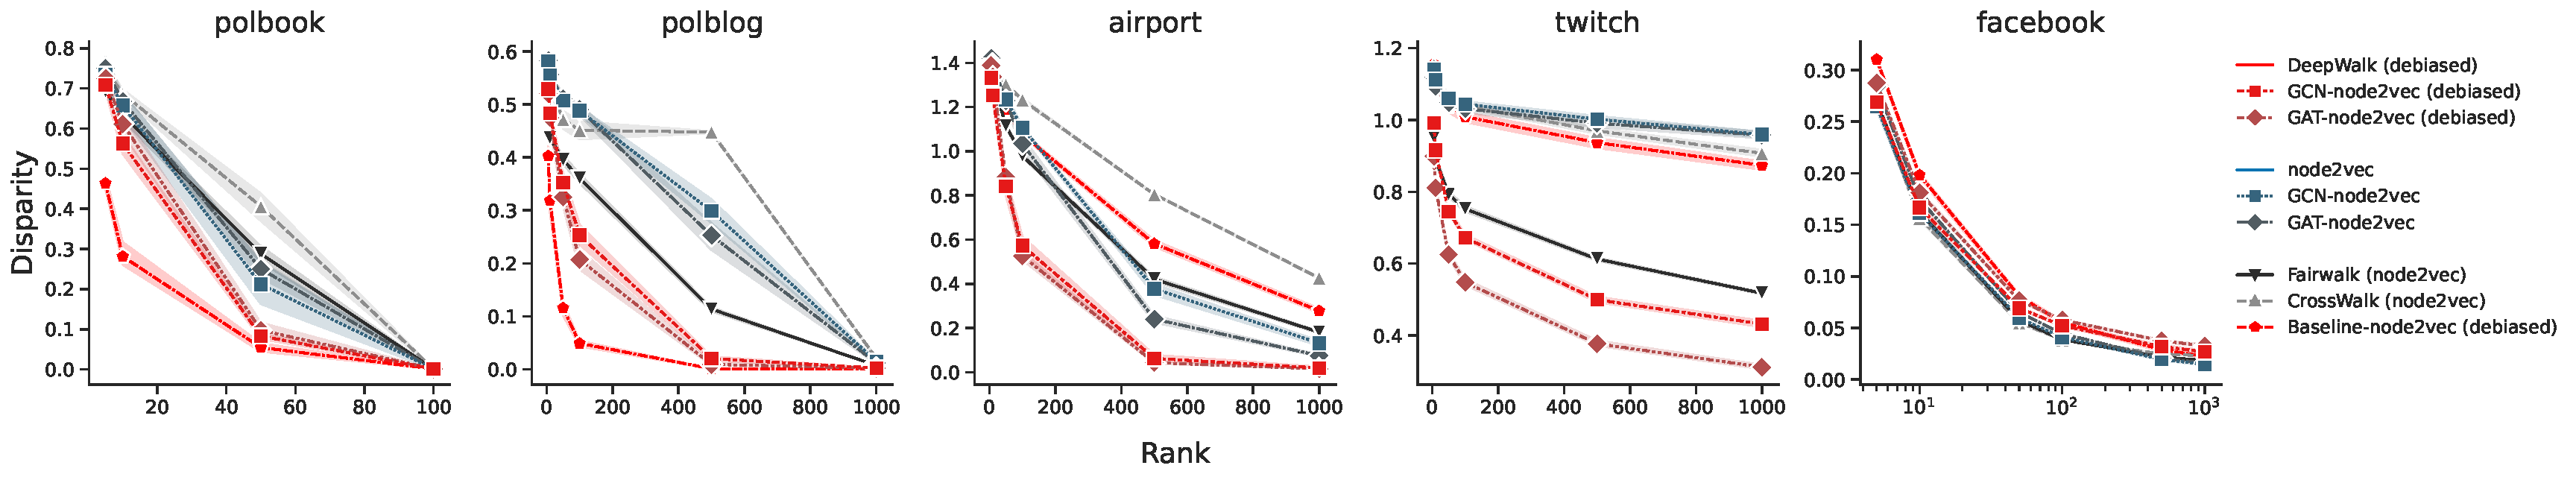
\includegraphics[width=\hsize]{images/disparity-curve_node2vec.pdf}
    \caption{Disparity with node2vec features}
    \label{fig:entropy_node2vec}
\end{figure*}
A demonstration of the proposed method on node2vec features is shown in Fig.\ref{fig:polbook-demonstration-appendix}. In this plot we show the stark difference between baseline and proposed method on two GNN architectures, GAT and GCN (two rows).
Here we have included PCA We can see that the proposed method can reduce the separability of the groups. 


\begin{figure*}[h]
    
    \begin{subfigure}[t]{\textwidth}
        
        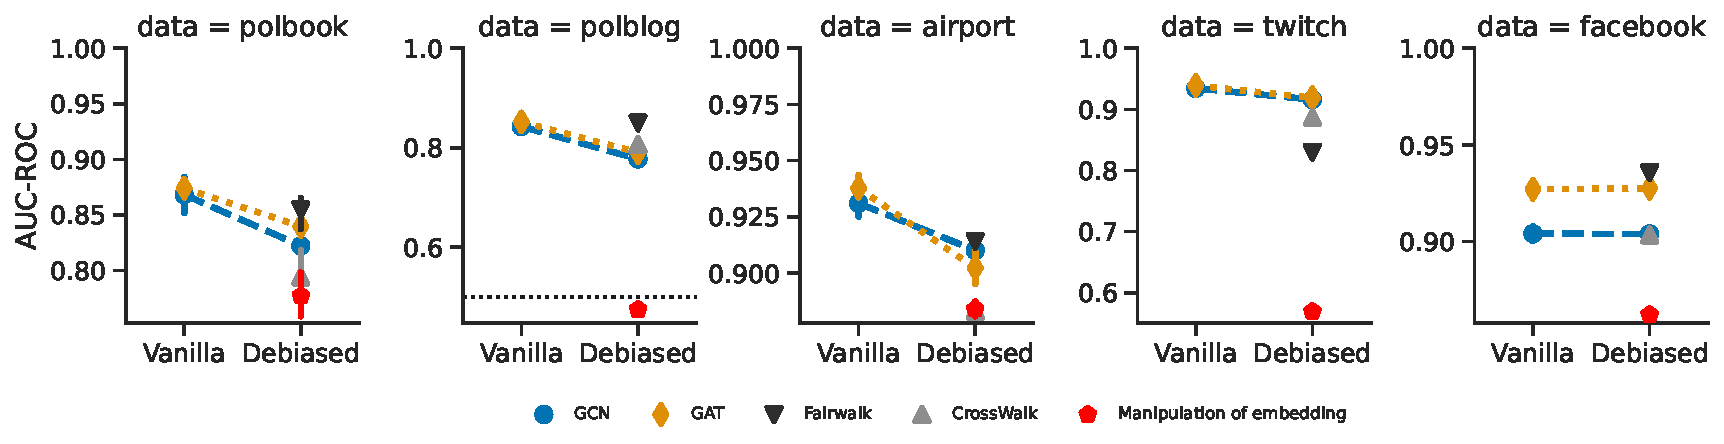
\includegraphics[width=.85\pdfpagewidth]{images/new_images/aucroc_node2vec.pdf}
        
        
        \label{fig:aucroc_node2vec}
    \end{subfigure}%
    
    \begin{subfigure}[t]{\textwidth}
        
        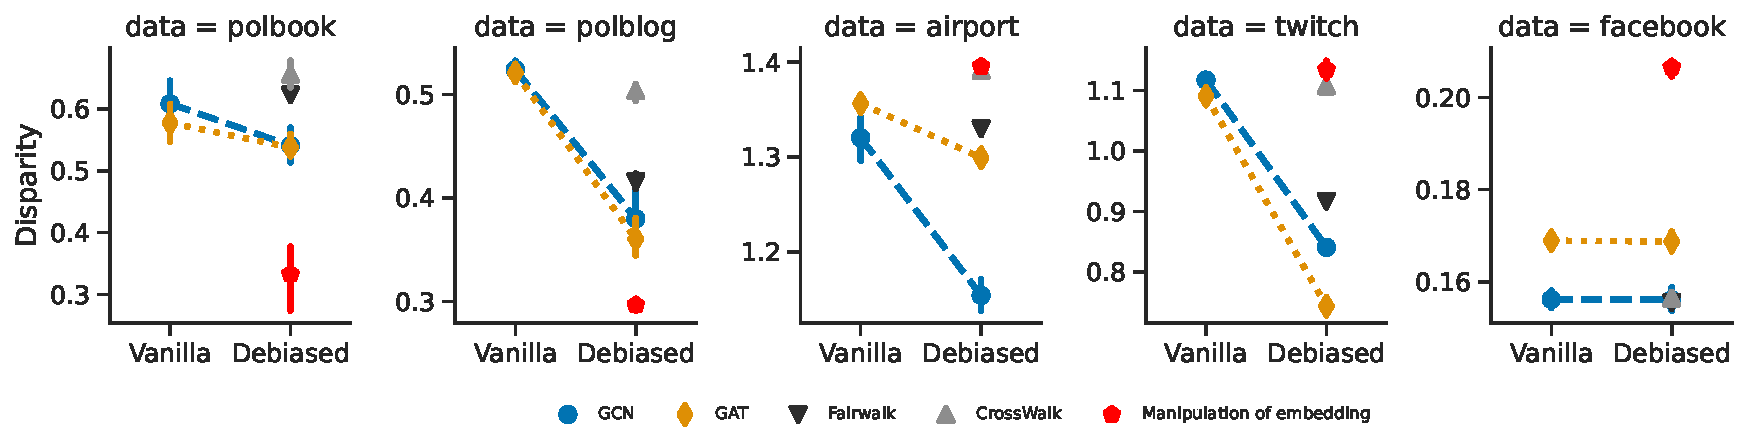
\includegraphics[width=.85 \pdfpagewidth]{images/new_images/disparity_node2vec.pdf}

        \label{fig:disparity_node2vec}
    \end{subfigure}%

  \caption{Link prediction (node2vec features)}
  \label{fig:sp_node2vec}
\end{figure*}

\subsection{Training Hyperparameters}

All graph neural networks take $128$ dimensional node features generated by DeepWalk/node2vec as input. Size of the neural network is different for different datasets. For smaller networks (Airport, Political Blogs and Political Book) we use 3 layers for GCNConv or GATConv stacked over one another, for Facebook 4 and for Twitch we use 5 followed by 2 linear layers. For different experiments, these DeepWalk/node2vec features are generated independently from different training networks. 
In cases of CrossWalk and Fairwalk, the training network is first modified using these algorithms and then a node2vec or DeepWalk model is trained to output a result of $128$ dimensional embeddings. Thus result of all the models (GNNs, CrossWalk, Fairwalk, DeepWalk/Fairwalk as baseline) are embeddings of $128$ dimensions for each node.

For Fairwalk, we train a random walk sampler for $1$ epoch with a window length of $10$ and walk length of $40$. In case of CrossWalk there are two important hyperparameters, $\alpha$ and $p$ which are used to modify the training network. For $\alpha$ we use a value of $0.7$ while for $p$ it is $2$. $\alpha$ is the multiplicating factor in the reweighting process. It controls the probability of a boundary node connected to other groups. This value is proportional to the number of inter-group connections in the resulting network. $p$ is the exponent in the reweighting process. It controls the amount of information that propagates from one group to other groups. The higher the value of $p$, the more is the information flow. For DeepWalk and node2vec we use $1$ epoch of training with a window length of $10$.

For GNNs we use either $3$, $4$ or $5$ layers of GATConv or GCNConv (depending on the dataset) stacked over one another. Output of each of those hidden layers is $64$ dimensional. The output of the model is a $128$ dimensional embedding of each node. For GATs we use $2$ heads in each GATConv layer. A dropout of $0.2$ is performed on the output of these layers before these are fed into a sequential module of two linear layers output of which is the embedding of the node. 

These models are trained using Adam optimizer with a learning rate of $0.001$ ($\frac{0.001}{32}$ for Twitch) and early stopping is used to prevent overfitting. Early stopping is configured to stop training when more than half of the batches reach a loss of zero. The model is trained for $300$ epochs for Airport, $600$ epochs for Political Book and Political Blogs datasets, $30$ for Facebook and $20$ for Twitch.  The model is trained on a GPU with a batch size of $256$ ($8$ for Twitch). Tesla A 100s were used to train all the models, with PyTorch being the machine learning tool of choice.
\begin{figure}%
    \centering
    \subfloat[\centering Local Fairness]{{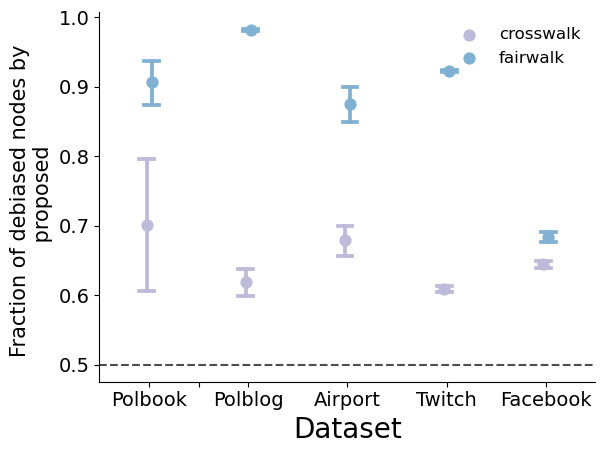
\includegraphics[width=.35\pdfpagewidth]{images/new_images/deepwalk_disparity_per_node_cw.png} }}%
    \qquad
    \subfloat[\centering Global Fairness]{{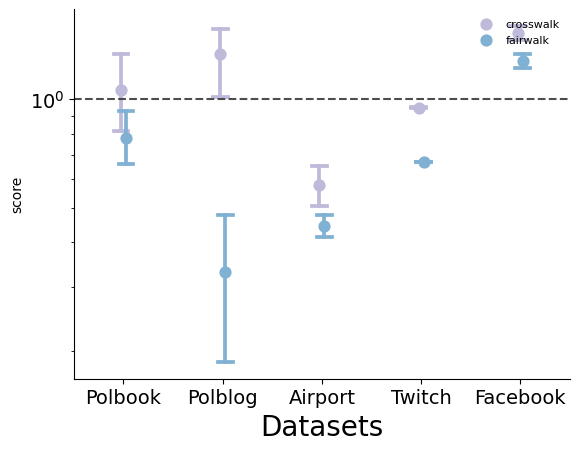
\includegraphics[width=.35\pdfpagewidth]{images/new_images/deepwalk_disparity_per_node_global_cw.png} }}%
    \caption{Comparison of Crosswalk and Fairwalk with vanilla deepwalk}%
    \label{fig:cw_fw_deepwalk}%
\end{figure}

\end{document}


% This document was modified from the file originally made available by
% Pat Langley and Andrea Danyluk for ICML-2K. This version was created
% by Iain Murray in 2018, and modified by Alexandre Bouchard in
% 2019 and 2021 and by Csaba Szepesvari, Gang Niu and Sivan Sabato in 2022.
% Modified again in 2023 by Sivan Sabato and Jonathan Scarlett.
% Previous contributors include Dan Roy, Lise Getoor and Tobias
% Scheffer, which was slightly modified from the 2010 version by
% Thorsten Joachims & Johannes Fuernkranz, slightly modified from the
% 2009 version by Kiri Wagstaff and Sam Roweis's 2008 version, which is
% slightly modified from Prasad Tadepalli's 2007 version which is a
% lightly changed version of the previous year's version by Andrew
% Moore, which was in turn edited from those of Kristian Kersting and
% Codrina Lauth. Alex Smola contributed to the algorithmic style files.

